\documentclass[1p]{elsarticle_modified}
%\bibliographystyle{elsarticle-num}

%\usepackage[colorlinks]{hyperref}
%\usepackage{abbrmath_seonhwa} %\Abb, \Ascr, \Acal ,\Abf, \Afrak
\usepackage{amsfonts}
\usepackage{amssymb}
\usepackage{amsmath}
\usepackage{amsthm}
\usepackage{scalefnt}
\usepackage{amsbsy}
\usepackage{kotex}
\usepackage{caption}
\usepackage{subfig}
\usepackage{color}
\usepackage{graphicx}
\usepackage{xcolor} %% white, black, red, green, blue, cyan, magenta, yellow
\usepackage{float}
\usepackage{setspace}
\usepackage{hyperref}

\usepackage{tikz}
\usetikzlibrary{arrows}

\usepackage{multirow}
\usepackage{array} % fixed length table
\usepackage{hhline}

%%%%%%%%%%%%%%%%%%%%%
\makeatletter
\renewcommand*\env@matrix[1][\arraystretch]{%
	\edef\arraystretch{#1}%
	\hskip -\arraycolsep
	\let\@ifnextchar\new@ifnextchar
	\array{*\c@MaxMatrixCols c}}
\makeatother %https://tex.stackexchange.com/questions/14071/how-can-i-increase-the-line-spacing-in-a-matrix
%%%%%%%%%%%%%%%

\usepackage[normalem]{ulem}

\newcommand{\msout}[1]{\ifmmode\text{\sout{\ensuremath{#1}}}\else\sout{#1}\fi}
%SOURCE: \msout is \stkout macro in https://tex.stackexchange.com/questions/20609/strikeout-in-math-mode

\newcommand{\cancel}[1]{
	\ifmmode
	{\color{red}\msout{#1}}
	\else
	{\color{red}\sout{#1}}
	\fi
}

\newcommand{\add}[1]{
	{\color{blue}\uwave{#1}}
}

\newcommand{\replace}[2]{
	\ifmmode
	{\color{red}\msout{#1}}{\color{blue}\uwave{#2}}
	\else
	{\color{red}\sout{#1}}{\color{blue}\uwave{#2}}
	\fi
}

\newcommand{\Sol}{\mathcal{S}} %segment
\newcommand{\D}{D} %diagram
\newcommand{\A}{\mathcal{A}} %arc


%%%%%%%%%%%%%%%%%%%%%%%%%%%%%5 test

\def\sl{\operatorname{\textup{SL}}(2,\Cbb)}
\def\psl{\operatorname{\textup{PSL}}(2,\Cbb)}
\def\quan{\mkern 1mu \triangleright \mkern 1mu}

\theoremstyle{definition}
\newtheorem{thm}{Theorem}[section]
\newtheorem{prop}[thm]{Proposition}
\newtheorem{lem}[thm]{Lemma}
\newtheorem{ques}[thm]{Question}
\newtheorem{cor}[thm]{Corollary}
\newtheorem{defn}[thm]{Definition}
\newtheorem{exam}[thm]{Example}
\newtheorem{rmk}[thm]{Remark}
\newtheorem{alg}[thm]{Algorithm}

\newcommand{\I}{\sqrt{-1}}
\begin{document}

%\begin{frontmatter}
%
%\title{Boundary parabolic representations of knots up to 8 crossings}
%
%%% Group authors per affiliation:
%\author{Yunhi Cho} 
%\address{Department of Mathematics, University of Seoul, Seoul, Korea}
%\ead{yhcho@uos.ac.kr}
%
%
%\author{Seonhwa Kim} %\fnref{s_kim}}
%\address{Center for Geometry and Physics, Institute for Basic Science, Pohang, 37673, Korea}
%\ead{ryeona17@ibs.re.kr}
%
%\author{Hyuk Kim}
%\address{Department of Mathematical Sciences, Seoul National University, Seoul 08826, Korea}
%\ead{hyukkim@snu.ac.kr}
%
%\author{Seokbeom Yoon}
%\address{Department of Mathematical Sciences, Seoul National University, Seoul, 08826,  Korea}
%\ead{sbyoon15@snu.ac.kr}
%
%\begin{abstract}
%We find all boundary parabolic representation of knots up to 8 crossings.
%
%\end{abstract}
%\begin{keyword}
%    \MSC[2010] 57M25 
%\end{keyword}
%
%\end{frontmatter}

%\linenumbers
%\tableofcontents
%
\newcommand\colored[1]{\textcolor{white}{\rule[-0.35ex]{0.8em}{1.4ex}}\kern-0.8em\color{red} #1}%
%\newcommand\colored[1]{\textcolor{white}{ #1}\kern-2.17ex	\textcolor{white}{ #1}\kern-1.81ex	\textcolor{white}{ #1}\kern-2.15ex\color{red}#1	}

{\Large $\underline{12n_{0299}~(K12n_{0299})}$}

\setlength{\tabcolsep}{10pt}
\renewcommand{\arraystretch}{1.6}
\vspace{1cm}\begin{tabular}{m{100pt}>{\centering\arraybackslash}m{274pt}}
\multirow{5}{120pt}{
	\centering
	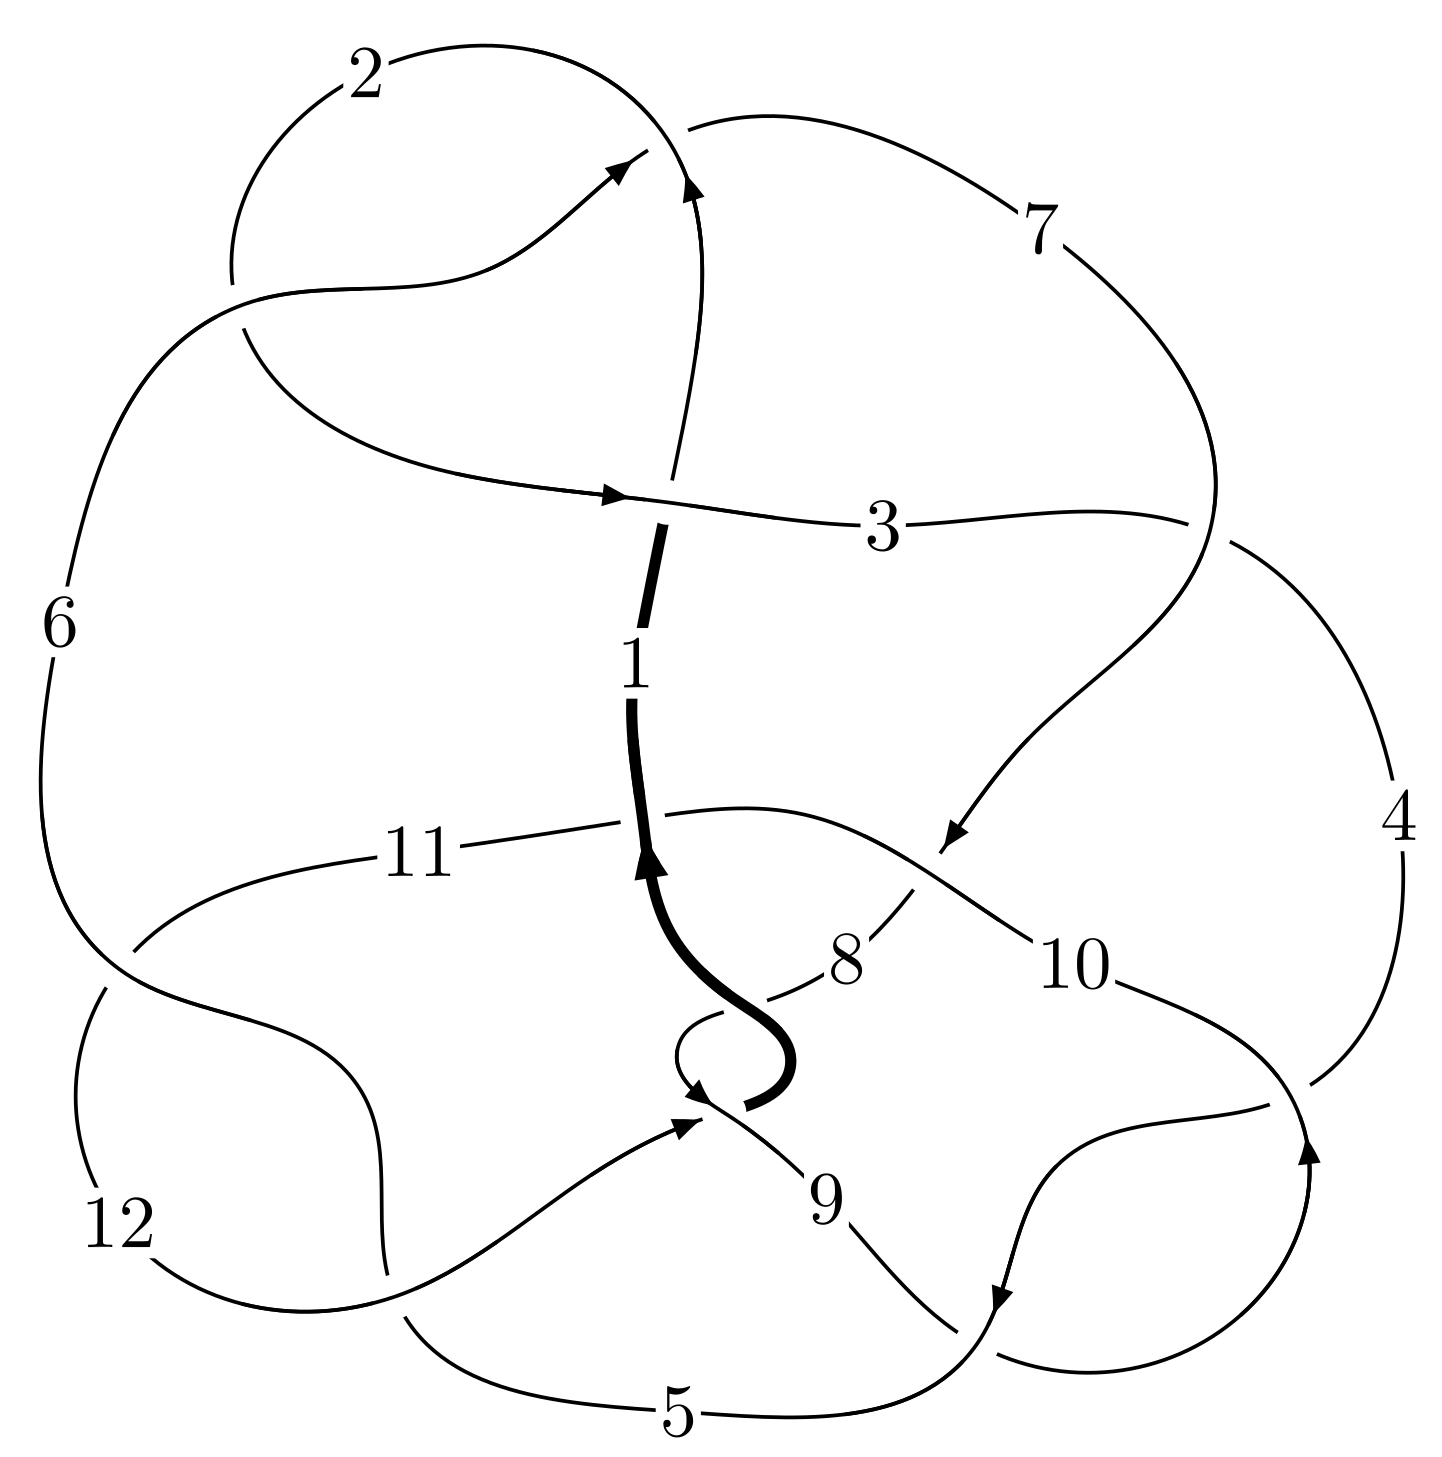
\includegraphics[width=112pt]{../../../GIT/diagram.site/Diagrams/png/2388_12n_0299.png}\\
\ \ \ A knot diagram\footnotemark}&
\allowdisplaybreaks
\textbf{Linearized knot diagam} \\
\cline{2-2}
 &
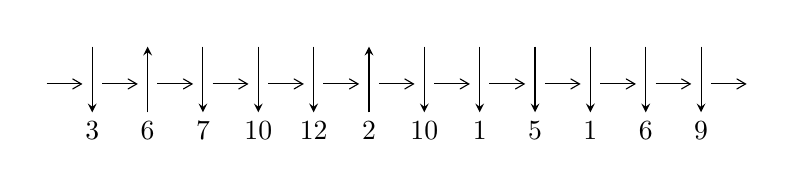
\begin{tikzpicture}[x=20pt, y=17pt]
	% nodes
	\node (C0) at (0, 0) {};
	\node (C1) at (1, 0) {};
	\node (C1U) at (1, +1) {};
	\node (C1D) at (1, -1) {3};

	\node (C2) at (2, 0) {};
	\node (C2U) at (2, +1) {};
	\node (C2D) at (2, -1) {6};

	\node (C3) at (3, 0) {};
	\node (C3U) at (3, +1) {};
	\node (C3D) at (3, -1) {7};

	\node (C4) at (4, 0) {};
	\node (C4U) at (4, +1) {};
	\node (C4D) at (4, -1) {10};

	\node (C5) at (5, 0) {};
	\node (C5U) at (5, +1) {};
	\node (C5D) at (5, -1) {12};

	\node (C6) at (6, 0) {};
	\node (C6U) at (6, +1) {};
	\node (C6D) at (6, -1) {2};

	\node (C7) at (7, 0) {};
	\node (C7U) at (7, +1) {};
	\node (C7D) at (7, -1) {10};

	\node (C8) at (8, 0) {};
	\node (C8U) at (8, +1) {};
	\node (C8D) at (8, -1) {1};

	\node (C9) at (9, 0) {};
	\node (C9U) at (9, +1) {};
	\node (C9D) at (9, -1) {5};

	\node (C10) at (10, 0) {};
	\node (C10U) at (10, +1) {};
	\node (C10D) at (10, -1) {1};

	\node (C11) at (11, 0) {};
	\node (C11U) at (11, +1) {};
	\node (C11D) at (11, -1) {6};

	\node (C12) at (12, 0) {};
	\node (C12U) at (12, +1) {};
	\node (C12D) at (12, -1) {9};
	\node (C13) at (13, 0) {};

	% arrows
	\draw[->,>={angle 60}]
	(C0) edge (C1) (C1) edge (C2) (C2) edge (C3) (C3) edge (C4) (C4) edge (C5) (C5) edge (C6) (C6) edge (C7) (C7) edge (C8) (C8) edge (C9) (C9) edge (C10) (C10) edge (C11) (C11) edge (C12) (C12) edge (C13) ;	\draw[->,>=stealth]
	(C1U) edge (C1D) (C2D) edge (C2U) (C3U) edge (C3D) (C4U) edge (C4D) (C5U) edge (C5D) (C6D) edge (C6U) (C7U) edge (C7D) (C8U) edge (C8D) (C9U) edge (C9D) (C10U) edge (C10D) (C11U) edge (C11D) (C12U) edge (C12D) ;
	\end{tikzpicture} \\
\hhline{~~} \\& 
\textbf{Solving Sequence} \\ \cline{2-2} 
 &
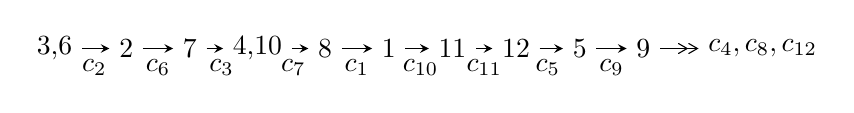
\begin{tikzpicture}[x=23pt, y=7pt]
	% node
	\node (A0) at (-1/8, 0) {3,6};
	\node (A1) at (1, 0) {2};
	\node (A2) at (2, 0) {7};
	\node (A3) at (49/16, 0) {4,10};
	\node (A4) at (33/8, 0) {8};
	\node (A5) at (41/8, 0) {1};
	\node (A6) at (49/8, 0) {11};
	\node (A7) at (57/8, 0) {12};
	\node (A8) at (65/8, 0) {5};
	\node (A9) at (73/8, 0) {9};
	\node (C1) at (1/2, -1) {$c_{2}$};
	\node (C2) at (3/2, -1) {$c_{6}$};
	\node (C3) at (5/2, -1) {$c_{3}$};
	\node (C4) at (29/8, -1) {$c_{7}$};
	\node (C5) at (37/8, -1) {$c_{1}$};
	\node (C6) at (45/8, -1) {$c_{10}$};
	\node (C7) at (53/8, -1) {$c_{11}$};
	\node (C8) at (61/8, -1) {$c_{5}$};
	\node (C9) at (69/8, -1) {$c_{9}$};
	\node (A10) at (11, 0) {$c_{4},c_{8},c_{12}$};

	% edge
	\draw[->,>=stealth]	
	(A0) edge (A1) (A1) edge (A2) (A2) edge (A3) (A3) edge (A4) (A4) edge (A5) (A5) edge (A6) (A6) edge (A7) (A7) edge (A8) (A8) edge (A9) ;
	\draw[->>,>={angle 60}]	
	(A9) edge (A10);
\end{tikzpicture} \\ 

\end{tabular} \\

\footnotetext{
The image of knot diagram is generated by the software ``\textbf{Draw programme}" developed by Andrew Bartholomew(\url{http://www.layer8.co.uk/maths/draw/index.htm\#Running-draw}), where we modified some parts for our purpose(\url{https://github.com/CATsTAILs/LinksPainter}).
}\phantom \\ \newline 
\centering \textbf{Ideals for irreducible components\footnotemark of $X_{\text{par}}$} 
 
\begin{align*}
I^u_{1}&=\langle 
-5 u^{28}-22 u^{27}+\cdots+2 b+4,\;- u^{28}- u^{27}+\cdots+2 a-5,\;u^{29}+6 u^{28}+\cdots-10 u-4\rangle \\
I^u_{2}&=\langle 
-123 u^7 a^3+644 u^7 a^2+\cdots-2637 a-1781,\;- u^7 a^3- u^7 a^2+\cdots+4 a-1,\\
\phantom{I^u_{2}}&\phantom{= \langle  }u^8- u^7+3 u^6-2 u^5+3 u^4-2 u^3-1\rangle \\
I^u_{3}&=\langle 
u^{18}- u^{17}+\cdots+b+1,\\
\phantom{I^u_{3}}&\phantom{= \langle  }u^{18}+5 u^{16}+u^{15}+12 u^{14}+3 u^{13}+15 u^{12}+4 u^{11}+8 u^{10}-3 u^8-4 u^7-5 u^6-4 u^5- u^4+u^2+a- u-1,\\
\phantom{I^u_{3}}&\phantom{= \langle  }u^{19}- u^{18}+\cdots+u-1\rangle \\
\\
\end{align*}
\raggedright * 3 irreducible components of $\dim_{\mathbb{C}}=0$, with total 80 representations.\\
\footnotetext{All coefficients of polynomials are rational numbers. But the coefficients are sometimes approximated in decimal forms when there is not enough margin.}
\newpage
\renewcommand{\arraystretch}{1}
\centering \section*{I. $I^u_{1}= \langle -5 u^{28}-22 u^{27}+\cdots+2 b+4,\;- u^{28}- u^{27}+\cdots+2 a-5,\;u^{29}+6 u^{28}+\cdots-10 u-4 \rangle$}
\flushleft \textbf{(i) Arc colorings}\\
\begin{tabular}{m{7pt} m{180pt} m{7pt} m{180pt} }
\flushright $a_{3}=$&$\begin{pmatrix}1\\0\end{pmatrix}$ \\
\flushright $a_{6}=$&$\begin{pmatrix}0\\u\end{pmatrix}$ \\
\flushright $a_{2}=$&$\begin{pmatrix}1\\u^2\end{pmatrix}$ \\
\flushright $a_{7}=$&$\begin{pmatrix}u\\u^3+u\end{pmatrix}$ \\
\flushright $a_{4}=$&$\begin{pmatrix}u^4+u^2+1\\u^6+2 u^4+u^2\end{pmatrix}$ \\
\flushright $a_{10}=$&$\begin{pmatrix}\frac{1}{2} u^{28}+\frac{1}{2} u^{27}+\cdots+2 u+\frac{5}{2}\\\frac{5}{2} u^{28}+11 u^{27}+\cdots-\frac{15}{2} u-2\end{pmatrix}$ \\
\flushright $a_{8}=$&$\begin{pmatrix}-\frac{3}{4} u^{28}-5 u^{27}+\cdots+\frac{71}{4} u+18\\\frac{1}{2} u^{28}+6 u^{27}+\cdots-\frac{19}{2} u+3\end{pmatrix}$ \\
\flushright $a_{1}=$&$\begin{pmatrix}u^2+1\\u^2\end{pmatrix}$ \\
\flushright $a_{11}=$&$\begin{pmatrix}- u^{28}-\frac{9}{2} u^{27}+\cdots+\frac{21}{2} u+\frac{21}{2}\\\frac{5}{2} u^{28}+15 u^{27}+\cdots-\frac{27}{2} u-2\end{pmatrix}$ \\
\flushright $a_{12}=$&$\begin{pmatrix}- u^{28}-\frac{9}{2} u^{27}+\cdots+\frac{21}{2} u+\frac{21}{2}\\-\frac{5}{2} u^{28}-8 u^{27}+\cdots-\frac{5}{2} u+4\end{pmatrix}$ \\
\flushright $a_{5}=$&$\begin{pmatrix}-\frac{3}{4} u^{28}-4 u^{27}+\cdots+\frac{19}{4} u+3\\-\frac{1}{2} u^{28}-3 u^{27}+\cdots+\frac{11}{2} u+3\end{pmatrix}$ \\
\flushright $a_{9}=$&$\begin{pmatrix}-\frac{1}{4} u^{28}- u^{27}+\cdots+\frac{5}{4} u+1\\-\frac{5}{2} u^{28}-11 u^{27}+\cdots+\frac{9}{2} u+3\end{pmatrix}$\\&\end{tabular}
\flushleft \textbf{(ii) Obstruction class $= -1$}\\~\\
\flushleft \textbf{(iii) Cusp Shapes $= u^{28}+6 u^{27}+26 u^{26}+78 u^{25}+195 u^{24}+404 u^{23}+742 u^{22}+1212 u^{21}+1814 u^{20}+2496 u^{19}+3192 u^{18}+3810 u^{17}+4264 u^{16}+4505 u^{15}+4511 u^{14}+4302 u^{13}+3916 u^{12}+3391 u^{11}+2793 u^{10}+2164 u^9+1573 u^8+1049 u^7+629 u^6+320 u^5+122 u^4+16 u^3-19 u^2-14 u-10$}\\~\\
\newpage\renewcommand{\arraystretch}{1}
\flushleft \textbf{(iv) u-Polynomials at the component}\newline \\
\begin{tabular}{m{50pt}|m{274pt}}
Crossings & \hspace{64pt}u-Polynomials at each crossing \\
\hline $$\begin{aligned}c_{1}\end{aligned}$$&$\begin{aligned}
&u^{29}+16 u^{28}+\cdots+108 u-16
\end{aligned}$\\
\hline $$\begin{aligned}c_{2},c_{6}\end{aligned}$$&$\begin{aligned}
&u^{29}-6 u^{28}+\cdots-10 u+4
\end{aligned}$\\
\hline $$\begin{aligned}c_{3}\end{aligned}$$&$\begin{aligned}
&u^{29}+6 u^{28}+\cdots+102 u+52
\end{aligned}$\\
\hline $$\begin{aligned}c_{4},c_{5},c_{9}\\c_{11}\end{aligned}$$&$\begin{aligned}
&u^{29}+7 u^{27}+\cdots+2 u+1
\end{aligned}$\\
\hline $$\begin{aligned}c_{7},c_{10}\end{aligned}$$&$\begin{aligned}
&u^{29}-3 u^{28}+\cdots-21 u+1
\end{aligned}$\\
\hline $$\begin{aligned}c_{8},c_{12}\end{aligned}$$&$\begin{aligned}
&u^{29}+19 u^{28}+\cdots+2304 u+256
\end{aligned}$\\
\hline
\end{tabular}\\~\\
\newpage\renewcommand{\arraystretch}{1}
\flushleft \textbf{(v) Riley Polynomials at the component}\newline \\
\begin{tabular}{m{50pt}|m{274pt}}
Crossings & \hspace{64pt}Riley Polynomials at each crossing \\
\hline $$\begin{aligned}c_{1}\end{aligned}$$&$\begin{aligned}
&y^{29}-4 y^{28}+\cdots+28400 y-256
\end{aligned}$\\
\hline $$\begin{aligned}c_{2},c_{6}\end{aligned}$$&$\begin{aligned}
&y^{29}+16 y^{28}+\cdots+108 y-16
\end{aligned}$\\
\hline $$\begin{aligned}c_{3}\end{aligned}$$&$\begin{aligned}
&y^{29}-24 y^{28}+\cdots+12588 y-2704
\end{aligned}$\\
\hline $$\begin{aligned}c_{4},c_{5},c_{9}\\c_{11}\end{aligned}$$&$\begin{aligned}
&y^{29}+14 y^{28}+\cdots-10 y-1
\end{aligned}$\\
\hline $$\begin{aligned}c_{7},c_{10}\end{aligned}$$&$\begin{aligned}
&y^{29}-49 y^{28}+\cdots+83 y-1
\end{aligned}$\\
\hline $$\begin{aligned}c_{8},c_{12}\end{aligned}$$&$\begin{aligned}
&y^{29}+9 y^{28}+\cdots+131072 y-65536
\end{aligned}$\\
\hline
\end{tabular}\\~\\
\newpage\flushleft \textbf{(vi) Complex Volumes and Cusp Shapes}
$$\begin{array}{c|c|c}  
\text{Solutions to }I^u_{1}& \I (\text{vol} + \sqrt{-1}CS) & \text{Cusp shape}\\
 \hline 
\begin{aligned}
u &= \phantom{-}0.529936 + 0.817458 I \\
a &= \phantom{-}0.234233 + 0.574816 I \\
b &= \phantom{-}0.345760 - 0.496091 I\end{aligned}
 & -1.24507 + 2.13242 I & -1.54126 - 5.97211 I \\ \hline\begin{aligned}
u &= \phantom{-}0.529936 - 0.817458 I \\
a &= \phantom{-}0.234233 - 0.574816 I \\
b &= \phantom{-}0.345760 + 0.496091 I\end{aligned}
 & -1.24507 - 2.13242 I & -1.54126 + 5.97211 I \\ \hline\begin{aligned}
u &= -0.333397 + 0.883512 I \\
a &= -0.369414 + 0.421127 I \\
b &= \phantom{-}0.248910 + 0.466784 I\end{aligned}
 & -0.53686 - 1.47819 I & -4.90590 + 3.46156 I \\ \hline\begin{aligned}
u &= -0.333397 - 0.883512 I \\
a &= -0.369414 - 0.421127 I \\
b &= \phantom{-}0.248910 - 0.466784 I\end{aligned}
 & -0.53686 + 1.47819 I & -4.90590 - 3.46156 I \\ \hline\begin{aligned}
u &= \phantom{-}0.230674 + 1.031600 I \\
a &= \phantom{-}0.622836 - 0.242190 I \\
b &= -0.393514 - 0.586648 I\end{aligned}
 & -3.27588 + 2.17781 I & -14.9005 - 2.5155 I \\ \hline\begin{aligned}
u &= \phantom{-}0.230674 - 1.031600 I \\
a &= \phantom{-}0.622836 + 0.242190 I \\
b &= -0.393514 + 0.586648 I\end{aligned}
 & -3.27588 - 2.17781 I & -14.9005 + 2.5155 I \\ \hline\begin{aligned}
u &= \phantom{-}0.752784 + 0.560145 I \\
a &= \phantom{-}0.141867 - 0.328248 I \\
b &= -0.290661 + 0.167634 I\end{aligned}
 & \phantom{-}4.48557 - 3.54679 I & -5.06701 + 3.83669 I \\ \hline\begin{aligned}
u &= \phantom{-}0.752784 - 0.560145 I \\
a &= \phantom{-}0.141867 + 0.328248 I \\
b &= -0.290661 - 0.167634 I\end{aligned}
 & \phantom{-}4.48557 + 3.54679 I & -5.06701 - 3.83669 I \\ \hline\begin{aligned}
u &= -0.929027 + 0.116767 I \\
a &= -2.22411 + 0.15082 I \\
b &= -2.04864 + 0.39982 I\end{aligned}
 & -2.62991 + 9.91881 I & -5.74423 - 5.24249 I \\ \hline\begin{aligned}
u &= -0.929027 - 0.116767 I \\
a &= -2.22411 - 0.15082 I \\
b &= -2.04864 - 0.39982 I\end{aligned}
 & -2.62991 - 9.91881 I & -5.74423 + 5.24249 I\\
 \hline 
 \end{array}$$\newpage$$\begin{array}{c|c|c}  
\text{Solutions to }I^u_{1}& \I (\text{vol} + \sqrt{-1}CS) & \text{Cusp shape}\\
 \hline 
\begin{aligned}
u &= -0.755090 + 0.452937 I \\
a &= -0.606953 - 0.612743 I \\
b &= -0.735838 - 0.187764 I\end{aligned}
 & \phantom{-}4.01496 - 0.67489 I & -6.09853 + 2.29351 I \\ \hline\begin{aligned}
u &= -0.755090 - 0.452937 I \\
a &= -0.606953 + 0.612743 I \\
b &= -0.735838 + 0.187764 I\end{aligned}
 & \phantom{-}4.01496 + 0.67489 I & -6.09853 - 2.29351 I \\ \hline\begin{aligned}
u &= -0.864712 + 0.123739 I \\
a &= \phantom{-}2.27119 + 0.52125 I \\
b &= \phantom{-}2.02843 + 0.16969 I\end{aligned}
 & -4.98255 + 2.50011 I & -6.07998 - 2.74065 I \\ \hline\begin{aligned}
u &= -0.864712 - 0.123739 I \\
a &= \phantom{-}2.27119 - 0.52125 I \\
b &= \phantom{-}2.02843 - 0.16969 I\end{aligned}
 & -4.98255 - 2.50011 I & -6.07998 + 2.74065 I \\ \hline\begin{aligned}
u &= \phantom{-}0.018688 + 1.158270 I \\
a &= -0.390605 + 0.430620 I \\
b &= \phantom{-}0.506072 + 0.444376 I\end{aligned}
 & -1.41808 - 2.24811 I & -11.36469 + 3.43943 I \\ \hline\begin{aligned}
u &= \phantom{-}0.018688 - 1.158270 I \\
a &= -0.390605 - 0.430620 I \\
b &= \phantom{-}0.506072 - 0.444376 I\end{aligned}
 & -1.41808 + 2.24811 I & -11.36469 - 3.43943 I \\ \hline\begin{aligned}
u &= \phantom{-}0.643120 + 0.992128 I \\
a &= -0.240554 - 0.246860 I \\
b &= -0.090211 + 0.397421 I\end{aligned}
 & \phantom{-}3.21603 + 8.80773 I & -6.26763 - 8.83895 I \\ \hline\begin{aligned}
u &= \phantom{-}0.643120 - 0.992128 I \\
a &= -0.240554 + 0.246860 I \\
b &= -0.090211 - 0.397421 I\end{aligned}
 & \phantom{-}3.21603 - 8.80773 I & -6.26763 + 8.83895 I \\ \hline\begin{aligned}
u &= -0.593156 + 1.076560 I \\
a &= \phantom{-}0.559837 + 0.468168 I \\
b &= \phantom{-}0.836083 - 0.325004 I\end{aligned}
 & \phantom{-}2.16507 - 4.43085 I & -9.17518 + 3.77414 I \\ \hline\begin{aligned}
u &= -0.593156 - 1.076560 I \\
a &= \phantom{-}0.559837 - 0.468168 I \\
b &= \phantom{-}0.836083 + 0.325004 I\end{aligned}
 & \phantom{-}2.16507 + 4.43085 I & -9.17518 - 3.77414 I\\
 \hline 
 \end{array}$$\newpage$$\begin{array}{c|c|c}  
\text{Solutions to }I^u_{1}& \I (\text{vol} + \sqrt{-1}CS) & \text{Cusp shape}\\
 \hline 
\begin{aligned}
u &= -0.396847 + 1.258520 I \\
a &= \phantom{-}0.13510 - 1.71384 I \\
b &= -2.10328 - 0.85015 I\end{aligned}
 & -9.21490 - 1.83630 I & -10.54114 + 0.46853 I \\ \hline\begin{aligned}
u &= -0.396847 - 1.258520 I \\
a &= \phantom{-}0.13510 + 1.71384 I \\
b &= -2.10328 + 0.85015 I\end{aligned}
 & -9.21490 + 1.83630 I & -10.54114 - 0.46853 I \\ \hline\begin{aligned}
u &= -0.525425 + 1.223980 I \\
a &= -0.68573 - 1.73877 I \\
b &= -2.48851 - 0.07427 I\end{aligned}
 & -8.26868 - 7.55554 I & -8.73863 + 5.55556 I \\ \hline\begin{aligned}
u &= -0.525425 - 1.223980 I \\
a &= -0.68573 + 1.73877 I \\
b &= -2.48851 + 0.07427 I\end{aligned}
 & -8.26868 + 7.55554 I & -8.73863 - 5.55556 I \\ \hline\begin{aligned}
u &= -0.398180 + 1.298960 I \\
a &= \phantom{-}0.28856 + 1.51336 I \\
b &= \phantom{-}2.08069 + 0.22776 I\end{aligned}
 & -7.09003 + 5.31029 I & -9.76890 - 2.61442 I \\ \hline\begin{aligned}
u &= -0.398180 - 1.298960 I \\
a &= \phantom{-}0.28856 - 1.51336 I \\
b &= \phantom{-}2.08069 - 0.22776 I\end{aligned}
 & -7.09003 - 5.31029 I & -9.76890 + 2.61442 I \\ \hline\begin{aligned}
u &= -0.533945 + 1.252430 I \\
a &= \phantom{-}0.25821 + 1.84759 I \\
b &= \phantom{-}2.45185 + 0.66312 I\end{aligned}
 & -6.0854 - 15.1894 I & -8.50713 + 8.09278 I \\ \hline\begin{aligned}
u &= -0.533945 - 1.252430 I \\
a &= \phantom{-}0.25821 - 1.84759 I \\
b &= \phantom{-}2.45185 - 0.66312 I\end{aligned}
 & -6.0854 + 15.1894 I & -8.50713 - 8.09278 I \\ \hline\begin{aligned}
u &= \phantom{-}0.309156\phantom{ +0.000000I} \\
a &= -0.988933\phantom{ +0.000000I} \\
b &= \phantom{-}0.305734\phantom{ +0.000000I}\end{aligned}
 & -0.776150\phantom{ +0.000000I} & -12.5990\phantom{ +0.000000I}\\
 \hline 
 \end{array}$$\newpage\newpage\renewcommand{\arraystretch}{1}
\centering \section*{II. $I^u_{2}= \langle -123 u^7 a^3+644 u^7 a^2+\cdots-2637 a-1781,\;- u^7 a^3- u^7 a^2+\cdots+4 a-1,\;u^8- u^7+3 u^6-2 u^5+3 u^4-2 u^3-1 \rangle$}
\flushleft \textbf{(i) Arc colorings}\\
\begin{tabular}{m{7pt} m{180pt} m{7pt} m{180pt} }
\flushright $a_{3}=$&$\begin{pmatrix}1\\0\end{pmatrix}$ \\
\flushright $a_{6}=$&$\begin{pmatrix}0\\u\end{pmatrix}$ \\
\flushright $a_{2}=$&$\begin{pmatrix}1\\u^2\end{pmatrix}$ \\
\flushright $a_{7}=$&$\begin{pmatrix}u\\u^3+u\end{pmatrix}$ \\
\flushright $a_{4}=$&$\begin{pmatrix}u^4+u^2+1\\u^6+2 u^4+u^2\end{pmatrix}$ \\
\flushright $a_{10}=$&$\begin{pmatrix}a\\0.0617160 a^{3} u^{7}-0.323131 a^{2} u^{7}+\cdots+1.32313 a+0.893628\end{pmatrix}$ \\
\flushright $a_{8}=$&$\begin{pmatrix}-0.205218 a^{3} u^{7}+0.497240 a^{2} u^{7}+\cdots+0.502760 a-2.00401\\0.0145509 a^{3} u^{7}+0.517311 a^{2} u^{7}+\cdots-1.51731 a-1.06573\end{pmatrix}$ \\
\flushright $a_{1}=$&$\begin{pmatrix}u^2+1\\u^2\end{pmatrix}$ \\
\flushright $a_{11}=$&$\begin{pmatrix}0.202208 a^{3} u^{7}-0.0180632 a^{2} u^{7}+\cdots+0.0180632 a-0.844456\\0.255896 a^{3} u^{7}-0.730055 a^{2} u^{7}+\cdots+1.73006 a+0.119920\end{pmatrix}$ \\
\flushright $a_{12}=$&$\begin{pmatrix}0.202208 a^{3} u^{7}-0.0180632 a^{2} u^{7}+\cdots+0.0180632 a-0.844456\\0.0842950 a^{3} u^{7}-0.416959 a^{2} u^{7}+\cdots+1.41696 a-1.24285\end{pmatrix}$ \\
\flushright $a_{5}=$&$\begin{pmatrix}-0.0496739 a^{3} u^{7}+0.406422 a^{2} u^{7}+\cdots-0.406422 a-0.499749\\0.308580 a^{3} u^{7}+1.38435 a^{2} u^{7}+\cdots+0.615655 a-4.53186\end{pmatrix}$ \\
\flushright $a_{9}=$&$\begin{pmatrix}-0.186653 a^{3} u^{7}+0.708981 a^{2} u^{7}+\cdots+1.29102 a-2.60512\\0.238334 a^{3} u^{7}+0.231811 a^{2} u^{7}+\cdots-1.23181 a-1.66282\end{pmatrix}$\\&\end{tabular}
\flushleft \textbf{(ii) Obstruction class $= -1$}\\~\\
\flushleft \textbf{(iii) Cusp Shapes $= -\frac{1636}{1993} u^7 a^3+\frac{3964}{1993} u^7 a^2+\cdots+\frac{4008}{1993} a-\frac{11990}{1993}$}\\~\\
\newpage\renewcommand{\arraystretch}{1}
\flushleft \textbf{(iv) u-Polynomials at the component}\newline \\
\begin{tabular}{m{50pt}|m{274pt}}
Crossings & \hspace{64pt}u-Polynomials at each crossing \\
\hline $$\begin{aligned}c_{1}\end{aligned}$$&$\begin{aligned}
&(u^8+5 u^7+11 u^6+10 u^5- u^4-10 u^3-6 u^2+1)^4
\end{aligned}$\\
\hline $$\begin{aligned}c_{2},c_{6}\end{aligned}$$&$\begin{aligned}
&(u^8+u^7+3 u^6+2 u^5+3 u^4+2 u^3-1)^4
\end{aligned}$\\
\hline $$\begin{aligned}c_{3}\end{aligned}$$&$\begin{aligned}
&(u^8- u^7-5 u^6+4 u^5+7 u^4-4 u^3-2 u^2+2 u-1)^4
\end{aligned}$\\
\hline $$\begin{aligned}c_{4},c_{5},c_{9}\\c_{11}\end{aligned}$$&$\begin{aligned}
&u^{32}- u^{31}+\cdots+830 u+361
\end{aligned}$\\
\hline $$\begin{aligned}c_{7},c_{10}\end{aligned}$$&$\begin{aligned}
&u^{32}-5 u^{31}+\cdots-27238 u+3169
\end{aligned}$\\
\hline $$\begin{aligned}c_{8},c_{12}\end{aligned}$$&$\begin{aligned}
&(u^2- u+1)^{16}
\end{aligned}$\\
\hline
\end{tabular}\\~\\
\newpage\renewcommand{\arraystretch}{1}
\flushleft \textbf{(v) Riley Polynomials at the component}\newline \\
\begin{tabular}{m{50pt}|m{274pt}}
Crossings & \hspace{64pt}Riley Polynomials at each crossing \\
\hline $$\begin{aligned}c_{1}\end{aligned}$$&$\begin{aligned}
&(y^8-3 y^7+19 y^6-34 y^5+71 y^4-66 y^3+34 y^2-12 y+1)^4
\end{aligned}$\\
\hline $$\begin{aligned}c_{2},c_{6}\end{aligned}$$&$\begin{aligned}
&(y^8+5 y^7+11 y^6+10 y^5- y^4-10 y^3-6 y^2+1)^4
\end{aligned}$\\
\hline $$\begin{aligned}c_{3}\end{aligned}$$&$\begin{aligned}
&(y^8-11 y^7+47 y^6-98 y^5+103 y^4-50 y^3+6 y^2+1)^4
\end{aligned}$\\
\hline $$\begin{aligned}c_{4},c_{5},c_{9}\\c_{11}\end{aligned}$$&$\begin{aligned}
&y^{32}+15 y^{31}+\cdots+1378908 y+130321
\end{aligned}$\\
\hline $$\begin{aligned}c_{7},c_{10}\end{aligned}$$&$\begin{aligned}
&y^{32}-21 y^{31}+\cdots+68151136 y+10042561
\end{aligned}$\\
\hline $$\begin{aligned}c_{8},c_{12}\end{aligned}$$&$\begin{aligned}
&(y^2+y+1)^{16}
\end{aligned}$\\
\hline
\end{tabular}\\~\\
\newpage\flushleft \textbf{(vi) Complex Volumes and Cusp Shapes}
$$\begin{array}{c|c|c}  
\text{Solutions to }I^u_{2}& \I (\text{vol} + \sqrt{-1}CS) & \text{Cusp shape}\\
 \hline 
\begin{aligned}
u &= \phantom{-}0.914675\phantom{ +0.000000I} \\
a &= \phantom{-}1.89629 + 0.39729 I \\
b &= \phantom{-}1.88389 + 0.10461 I\end{aligned}
 & -5.24109 - 2.02988 I & -5.82210 + 3.46410 I \\ \hline\begin{aligned}
u &= \phantom{-}0.914675\phantom{ +0.000000I} \\
a &= \phantom{-}1.89629 - 0.39729 I \\
b &= \phantom{-}1.88389 - 0.10461 I\end{aligned}
 & -5.24109 + 2.02988 I & -5.82210 - 3.46410 I \\ \hline\begin{aligned}
u &= \phantom{-}0.914675\phantom{ +0.000000I} \\
a &= -2.05963 + 0.11437 I \\
b &= -1.73449 + 0.36339 I\end{aligned}
 & -5.24109 + 2.02988 I & -5.82210 - 3.46410 I \\ \hline\begin{aligned}
u &= \phantom{-}0.914675\phantom{ +0.000000I} \\
a &= -2.05963 - 0.11437 I \\
b &= -1.73449 - 0.36339 I\end{aligned}
 & -5.24109 - 2.02988 I & -5.82210 + 3.46410 I \\ \hline\begin{aligned}
u &= \phantom{-}0.252896 + 0.819281 I \\
a &= \phantom{-}0.839815 + 0.637967 I \\
b &= \phantom{-}0.38233 + 2.21666 I\end{aligned}
 & \phantom{-}4.44352 - 0.75456 I & -3.18053 - 1.62107 I \\ \hline\begin{aligned}
u &= \phantom{-}0.252896 + 0.819281 I \\
a &= \phantom{-}1.61466 + 0.45267 I \\
b &= -1.49292 + 1.35353 I\end{aligned}
 & \phantom{-}4.44352 + 3.30520 I & -3.18053 - 8.54928 I \\ \hline\begin{aligned}
u &= \phantom{-}0.252896 + 0.819281 I \\
a &= -0.99481 - 2.12932 I \\
b &= -0.03748 - 1.43734 I\end{aligned}
 & \phantom{-}4.44352 + 3.30520 I & -3.18053 - 8.54928 I \\ \hline\begin{aligned}
u &= \phantom{-}0.252896 + 0.819281 I \\
a &= -2.60176 - 0.33644 I \\
b &= \phantom{-}0.310288 - 0.849384 I\end{aligned}
 & \phantom{-}4.44352 - 0.75456 I & -3.18053 - 1.62107 I \\ \hline\begin{aligned}
u &= \phantom{-}0.252896 - 0.819281 I \\
a &= \phantom{-}0.839815 - 0.637967 I \\
b &= \phantom{-}0.38233 - 2.21666 I\end{aligned}
 & \phantom{-}4.44352 + 0.75456 I & -3.18053 + 1.62107 I \\ \hline\begin{aligned}
u &= \phantom{-}0.252896 - 0.819281 I \\
a &= \phantom{-}1.61466 - 0.45267 I \\
b &= -1.49292 - 1.35353 I\end{aligned}
 & \phantom{-}4.44352 - 3.30520 I & -3.18053 + 8.54928 I\\
 \hline 
 \end{array}$$\newpage$$\begin{array}{c|c|c}  
\text{Solutions to }I^u_{2}& \I (\text{vol} + \sqrt{-1}CS) & \text{Cusp shape}\\
 \hline 
\begin{aligned}
u &= \phantom{-}0.252896 - 0.819281 I \\
a &= -0.99481 + 2.12932 I \\
b &= -0.03748 + 1.43734 I\end{aligned}
 & \phantom{-}4.44352 - 3.30520 I & -3.18053 + 8.54928 I \\ \hline\begin{aligned}
u &= \phantom{-}0.252896 - 0.819281 I \\
a &= -2.60176 + 0.33644 I \\
b &= \phantom{-}0.310288 + 0.849384 I\end{aligned}
 & \phantom{-}4.44352 + 0.75456 I & -3.18053 + 1.62107 I \\ \hline\begin{aligned}
u &= -0.394459 + 1.112500 I \\
a &= -0.559029 + 1.096920 I \\
b &= \phantom{-}0.095737 + 0.849097 I\end{aligned}
 & \phantom{-}0.58960 - 1.60295 I & -8.42240 + 1.05392 I \\ \hline\begin{aligned}
u &= -0.394459 + 1.112500 I \\
a &= -0.650891 + 0.316842 I \\
b &= \phantom{-}0.99981 + 1.05461 I\end{aligned}
 & \phantom{-}0.58960 - 1.60295 I & -8.42240 + 1.05392 I \\ \hline\begin{aligned}
u &= -0.394459 + 1.112500 I \\
a &= \phantom{-}1.265140 + 0.509213 I \\
b &= \phantom{-}0.035342 - 0.694019 I\end{aligned}
 & \phantom{-}0.58960 - 5.66272 I & -8.42240 + 7.98213 I \\ \hline\begin{aligned}
u &= -0.394459 + 1.112500 I \\
a &= \phantom{-}0.564174 - 0.168272 I \\
b &= \phantom{-}1.06554 - 1.20660 I\end{aligned}
 & \phantom{-}0.58960 - 5.66272 I & -8.42240 + 7.98213 I \\ \hline\begin{aligned}
u &= -0.394459 - 1.112500 I \\
a &= -0.559029 - 1.096920 I \\
b &= \phantom{-}0.095737 - 0.849097 I\end{aligned}
 & \phantom{-}0.58960 + 1.60295 I & -8.42240 - 1.05392 I \\ \hline\begin{aligned}
u &= -0.394459 - 1.112500 I \\
a &= -0.650891 - 0.316842 I \\
b &= \phantom{-}0.99981 - 1.05461 I\end{aligned}
 & \phantom{-}0.58960 + 1.60295 I & -8.42240 - 1.05392 I \\ \hline\begin{aligned}
u &= -0.394459 - 1.112500 I \\
a &= \phantom{-}1.265140 - 0.509213 I \\
b &= \phantom{-}0.035342 + 0.694019 I\end{aligned}
 & \phantom{-}0.58960 + 5.66272 I & -8.42240 - 7.98213 I \\ \hline\begin{aligned}
u &= -0.394459 - 1.112500 I \\
a &= \phantom{-}0.564174 + 0.168272 I \\
b &= \phantom{-}1.06554 + 1.20660 I\end{aligned}
 & \phantom{-}0.58960 + 5.66272 I & -8.42240 - 7.98213 I\\
 \hline 
 \end{array}$$\newpage$$\begin{array}{c|c|c}  
\text{Solutions to }I^u_{2}& \I (\text{vol} + \sqrt{-1}CS) & \text{Cusp shape}\\
 \hline 
\begin{aligned}
u &= \phantom{-}0.473514 + 1.273020 I \\
a &= -0.278598 + 1.324080 I \\
b &= -2.19588 + 0.14617 I\end{aligned}
 & -9.13765 + 2.90536 I & -8.98443 + 0.46988 I \\ \hline\begin{aligned}
u &= \phantom{-}0.473514 + 1.273020 I \\
a &= \phantom{-}0.15293 - 1.46513 I \\
b &= \phantom{-}2.23599 - 0.76370 I\end{aligned}
 & -9.13765 + 6.96513 I & -8.98443 - 6.45832 I \\ \hline\begin{aligned}
u &= \phantom{-}0.473514 + 1.273020 I \\
a &= \phantom{-}0.46276 - 1.55281 I \\
b &= \phantom{-}1.81750 - 0.27231 I\end{aligned}
 & -9.13765 + 2.90536 I & -8.98443 + 0.46988 I \\ \hline\begin{aligned}
u &= \phantom{-}0.473514 + 1.273020 I \\
a &= -0.04692 + 1.73899 I \\
b &= -1.93756 + 0.49908 I\end{aligned}
 & -9.13765 + 6.96513 I & -8.98443 - 6.45832 I \\ \hline\begin{aligned}
u &= \phantom{-}0.473514 - 1.273020 I \\
a &= -0.278598 - 1.324080 I \\
b &= -2.19588 - 0.14617 I\end{aligned}
 & -9.13765 - 2.90536 I & -8.98443 - 0.46988 I \\ \hline\begin{aligned}
u &= \phantom{-}0.473514 - 1.273020 I \\
a &= \phantom{-}0.15293 + 1.46513 I \\
b &= \phantom{-}2.23599 + 0.76370 I\end{aligned}
 & -9.13765 - 6.96513 I & -8.98443 + 6.45832 I \\ \hline\begin{aligned}
u &= \phantom{-}0.473514 - 1.273020 I \\
a &= \phantom{-}0.46276 + 1.55281 I \\
b &= \phantom{-}1.81750 + 0.27231 I\end{aligned}
 & -9.13765 - 2.90536 I & -8.98443 - 0.46988 I \\ \hline\begin{aligned}
u &= \phantom{-}0.473514 - 1.273020 I \\
a &= -0.04692 - 1.73899 I \\
b &= -1.93756 - 0.49908 I\end{aligned}
 & -9.13765 - 6.96513 I & -8.98443 + 6.45832 I \\ \hline\begin{aligned}
u &= -0.578577\phantom{ +0.000000I} \\
a &= -1.046970 + 0.657077 I \\
b &= -0.322351 + 1.227360 I\end{aligned}
 & \phantom{-}3.58052 - 2.02988 I & -5.00319 + 3.46410 I \\ \hline\begin{aligned}
u &= -0.578577\phantom{ +0.000000I} \\
a &= -1.046970 - 0.657077 I \\
b &= -0.322351 - 1.227360 I\end{aligned}
 & \phantom{-}3.58052 + 2.02988 I & -5.00319 - 3.46410 I\\
 \hline 
 \end{array}$$\newpage$$\begin{array}{c|c|c}  
\text{Solutions to }I^u_{2}& \I (\text{vol} + \sqrt{-1}CS) & \text{Cusp shape}\\
 \hline 
\begin{aligned}
u &= -0.578577\phantom{ +0.000000I} \\
a &= -0.55714 + 2.12134 I \\
b &= -0.605755 + 0.380170 I\end{aligned}
 & \phantom{-}3.58052 - 2.02988 I & -5.00319 + 3.46410 I \\ \hline\begin{aligned}
u &= -0.578577\phantom{ +0.000000I} \\
a &= -0.55714 - 2.12134 I \\
b &= -0.605755 - 0.380170 I\end{aligned}
 & \phantom{-}3.58052 + 2.02988 I & -5.00319 - 3.46410 I\\
 \hline 
 \end{array}$$\newpage\newpage\renewcommand{\arraystretch}{1}
\centering \section*{III. $I^u_{3}= \langle u^{18}- u^{17}+\cdots+b+1,\;u^{18}+5 u^{16}+\cdots+a-1,\;u^{19}- u^{18}+\cdots+u-1 \rangle$}
\flushleft \textbf{(i) Arc colorings}\\
\begin{tabular}{m{7pt} m{180pt} m{7pt} m{180pt} }
\flushright $a_{3}=$&$\begin{pmatrix}1\\0\end{pmatrix}$ \\
\flushright $a_{6}=$&$\begin{pmatrix}0\\u\end{pmatrix}$ \\
\flushright $a_{2}=$&$\begin{pmatrix}1\\u^2\end{pmatrix}$ \\
\flushright $a_{7}=$&$\begin{pmatrix}u\\u^3+u\end{pmatrix}$ \\
\flushright $a_{4}=$&$\begin{pmatrix}u^4+u^2+1\\u^6+2 u^4+u^2\end{pmatrix}$ \\
\flushright $a_{10}=$&$\begin{pmatrix}- u^{18}-5 u^{16}+\cdots+u+1\\- u^{18}+u^{17}+\cdots+2 u-1\end{pmatrix}$ \\
\flushright $a_{8}=$&$\begin{pmatrix}2 u^{18}-3 u^{17}+\cdots-4 u+2\\- u^{18}-4 u^{16}+\cdots+u+2\end{pmatrix}$ \\
\flushright $a_{1}=$&$\begin{pmatrix}u^2+1\\u^2\end{pmatrix}$ \\
\flushright $a_{11}=$&$\begin{pmatrix}- u^{18}-5 u^{16}+\cdots+u+1\\-2 u^{18}+2 u^{17}+\cdots+3 u-1\end{pmatrix}$ \\
\flushright $a_{12}=$&$\begin{pmatrix}- u^{18}-5 u^{16}+\cdots+u+1\\-2 u^{18}+2 u^{17}+\cdots+3 u-2\end{pmatrix}$ \\
\flushright $a_{5}=$&$\begin{pmatrix}- u^{18}+2 u^{17}+\cdots+4 u-2\\u^{18}- u^{17}+\cdots-2 u-1\end{pmatrix}$ \\
\flushright $a_{9}=$&$\begin{pmatrix}2 u^{18}-2 u^{17}+\cdots-4 u+1\\- u^{17}+u^{16}+\cdots- u+3\end{pmatrix}$\\&\end{tabular}
\flushleft \textbf{(ii) Obstruction class $= 1$}\\~\\
\flushleft \textbf{(iii) Cusp Shapes $= -2 u^{17}+3 u^{16}-11 u^{15}+15 u^{14}-28 u^{13}+35 u^{12}-39 u^{11}+41 u^{10}-30 u^9+20 u^8-10 u^7-4 u^6-3 u^5-5 u^3+8 u^2-3 u-2$}\\~\\
\newpage\renewcommand{\arraystretch}{1}
\flushleft \textbf{(iv) u-Polynomials at the component}\newline \\
\begin{tabular}{m{50pt}|m{274pt}}
Crossings & \hspace{64pt}u-Polynomials at each crossing \\
\hline $$\begin{aligned}c_{1}\end{aligned}$$&$\begin{aligned}
&u^{19}-11 u^{18}+\cdots-5 u+1
\end{aligned}$\\
\hline $$\begin{aligned}c_{2}\end{aligned}$$&$\begin{aligned}
&u^{19}- u^{18}+\cdots+u-1
\end{aligned}$\\
\hline $$\begin{aligned}c_{3}\end{aligned}$$&$\begin{aligned}
&u^{19}+u^{18}+\cdots- u-1
\end{aligned}$\\
\hline $$\begin{aligned}c_{4},c_{11}\end{aligned}$$&$\begin{aligned}
&u^{19}+8 u^{17}+\cdots+3 u-1
\end{aligned}$\\
\hline $$\begin{aligned}c_{5},c_{9}\end{aligned}$$&$\begin{aligned}
&u^{19}+8 u^{17}+\cdots+3 u+1
\end{aligned}$\\
\hline $$\begin{aligned}c_{6}\end{aligned}$$&$\begin{aligned}
&u^{19}+u^{18}+\cdots+u+1
\end{aligned}$\\
\hline $$\begin{aligned}c_{7},c_{10}\end{aligned}$$&$\begin{aligned}
&u^{19}-3 u^{18}+\cdots-2 u-1
\end{aligned}$\\
\hline $$\begin{aligned}c_{8}\end{aligned}$$&$\begin{aligned}
&u^{19}+2 u^{18}+\cdots+3 u-1
\end{aligned}$\\
\hline $$\begin{aligned}c_{12}\end{aligned}$$&$\begin{aligned}
&u^{19}-2 u^{18}+\cdots+3 u+1
\end{aligned}$\\
\hline
\end{tabular}\\~\\
\newpage\renewcommand{\arraystretch}{1}
\flushleft \textbf{(v) Riley Polynomials at the component}\newline \\
\begin{tabular}{m{50pt}|m{274pt}}
Crossings & \hspace{64pt}Riley Polynomials at each crossing \\
\hline $$\begin{aligned}c_{1}\end{aligned}$$&$\begin{aligned}
&y^{19}- y^{18}+\cdots- y-1
\end{aligned}$\\
\hline $$\begin{aligned}c_{2},c_{6}\end{aligned}$$&$\begin{aligned}
&y^{19}+11 y^{18}+\cdots-5 y-1
\end{aligned}$\\
\hline $$\begin{aligned}c_{3}\end{aligned}$$&$\begin{aligned}
&y^{19}-13 y^{18}+\cdots-11 y-1
\end{aligned}$\\
\hline $$\begin{aligned}c_{4},c_{5},c_{9}\\c_{11}\end{aligned}$$&$\begin{aligned}
&y^{19}+16 y^{18}+\cdots-21 y-1
\end{aligned}$\\
\hline $$\begin{aligned}c_{7},c_{10}\end{aligned}$$&$\begin{aligned}
&y^{19}-3 y^{18}+\cdots-8 y-1
\end{aligned}$\\
\hline $$\begin{aligned}c_{8},c_{12}\end{aligned}$$&$\begin{aligned}
&y^{19}+8 y^{18}+\cdots+3 y-1
\end{aligned}$\\
\hline
\end{tabular}\\~\\
\newpage\flushleft \textbf{(vi) Complex Volumes and Cusp Shapes}
$$\begin{array}{c|c|c}  
\text{Solutions to }I^u_{3}& \I (\text{vol} + \sqrt{-1}CS) & \text{Cusp shape}\\
 \hline 
\begin{aligned}
u &= -0.432409 + 0.844316 I \\
a &= -0.329441 + 0.448815 I \\
b &= -0.236489 - 0.472224 I\end{aligned}
 & -1.79244 - 1.81593 I & -13.41650 + 0.65086 I \\ \hline\begin{aligned}
u &= -0.432409 - 0.844316 I \\
a &= -0.329441 - 0.448815 I \\
b &= -0.236489 + 0.472224 I\end{aligned}
 & -1.79244 + 1.81593 I & -13.41650 - 0.65086 I \\ \hline\begin{aligned}
u &= \phantom{-}0.355611 + 1.040830 I \\
a &= \phantom{-}1.62344 + 0.58218 I \\
b &= -0.02864 + 1.89676 I\end{aligned}
 & \phantom{-}2.78146 - 0.05347 I & -7.84525 - 1.09777 I \\ \hline\begin{aligned}
u &= \phantom{-}0.355611 - 1.040830 I \\
a &= \phantom{-}1.62344 - 0.58218 I \\
b &= -0.02864 - 1.89676 I\end{aligned}
 & \phantom{-}2.78146 + 0.05347 I & -7.84525 + 1.09777 I \\ \hline\begin{aligned}
u &= \phantom{-}0.890704\phantom{ +0.000000I} \\
a &= -2.06630\phantom{ +0.000000I} \\
b &= -1.84047\phantom{ +0.000000I}\end{aligned}
 & -5.60220\phantom{ +0.000000I} & -6.95090\phantom{ +0.000000I} \\ \hline\begin{aligned}
u &= -0.326702 + 1.147210 I \\
a &= -0.125098 - 0.538940 I \\
b &= \phantom{-}0.659149 + 0.032559 I\end{aligned}
 & \phantom{-}1.46823 - 3.78813 I & -6.32142 + 3.96435 I \\ \hline\begin{aligned}
u &= -0.326702 - 1.147210 I \\
a &= -0.125098 + 0.538940 I \\
b &= \phantom{-}0.659149 - 0.032559 I\end{aligned}
 & \phantom{-}1.46823 + 3.78813 I & -6.32142 - 3.96435 I \\ \hline\begin{aligned}
u &= \phantom{-}0.536152 + 1.067450 I \\
a &= -1.382960 - 0.137280 I \\
b &= -0.59494 - 1.54985 I\end{aligned}
 & \phantom{-}4.08792 + 6.74742 I & -5.06014 - 6.00387 I \\ \hline\begin{aligned}
u &= \phantom{-}0.536152 - 1.067450 I \\
a &= -1.382960 + 0.137280 I \\
b &= -0.59494 + 1.54985 I\end{aligned}
 & \phantom{-}4.08792 - 6.74742 I & -5.06014 + 6.00387 I \\ \hline\begin{aligned}
u &= \phantom{-}0.101153 + 0.760282 I \\
a &= \phantom{-}1.81914 + 1.18798 I \\
b &= -0.71919 + 1.50323 I\end{aligned}
 & \phantom{-}4.29021 + 2.32381 I & -5.29787 - 0.37944 I\\
 \hline 
 \end{array}$$\newpage$$\begin{array}{c|c|c}  
\text{Solutions to }I^u_{3}& \I (\text{vol} + \sqrt{-1}CS) & \text{Cusp shape}\\
 \hline 
\begin{aligned}
u &= \phantom{-}0.101153 - 0.760282 I \\
a &= \phantom{-}1.81914 - 1.18798 I \\
b &= -0.71919 - 1.50323 I\end{aligned}
 & \phantom{-}4.29021 - 2.32381 I & -5.29787 + 0.37944 I \\ \hline\begin{aligned}
u &= -0.682478 + 0.327459 I \\
a &= -0.427115 + 0.321033 I \\
b &= \phantom{-}0.186371 - 0.358960 I\end{aligned}
 & \phantom{-}5.43330 - 0.84474 I & \phantom{-}0.382477 + 1.325719 I \\ \hline\begin{aligned}
u &= -0.682478 - 0.327459 I \\
a &= -0.427115 - 0.321033 I \\
b &= \phantom{-}0.186371 + 0.358960 I\end{aligned}
 & \phantom{-}5.43330 + 0.84474 I & \phantom{-}0.382477 - 1.325719 I \\ \hline\begin{aligned}
u &= -0.557218 + 1.113290 I \\
a &= \phantom{-}0.172420 + 0.230688 I \\
b &= -0.352897 + 0.063409 I\end{aligned}
 & \phantom{-}3.17508 - 3.96127 I & -2.77988 + 1.70184 I \\ \hline\begin{aligned}
u &= -0.557218 - 1.113290 I \\
a &= \phantom{-}0.172420 - 0.230688 I \\
b &= -0.352897 - 0.063409 I\end{aligned}
 & \phantom{-}3.17508 + 3.96127 I & -2.77988 - 1.70184 I \\ \hline\begin{aligned}
u &= \phantom{-}0.587141 + 0.436351 I \\
a &= -0.56266 - 1.67318 I \\
b &= \phantom{-}0.399733 - 1.227910 I\end{aligned}
 & \phantom{-}5.94319 - 2.22864 I & -0.25827 + 1.68244 I \\ \hline\begin{aligned}
u &= \phantom{-}0.587141 - 0.436351 I \\
a &= -0.56266 + 1.67318 I \\
b &= \phantom{-}0.399733 + 1.227910 I\end{aligned}
 & \phantom{-}5.94319 + 2.22864 I & -0.25827 - 1.68244 I \\ \hline\begin{aligned}
u &= \phantom{-}0.473398 + 1.262070 I \\
a &= \phantom{-}0.24543 - 1.57752 I \\
b &= \phantom{-}2.10713 - 0.43705 I\end{aligned}
 & -9.42638 + 4.85839 I & -9.92768 - 3.28951 I \\ \hline\begin{aligned}
u &= \phantom{-}0.473398 - 1.262070 I \\
a &= \phantom{-}0.24543 + 1.57752 I \\
b &= \phantom{-}2.10713 + 0.43705 I\end{aligned}
 & -9.42638 - 4.85839 I & -9.92768 + 3.28951 I\\
 \hline 
 \end{array}$$\newpage
\newpage\renewcommand{\arraystretch}{1}
\centering \section*{ IV. u-Polynomials}
\begin{tabular}{m{50pt}|m{274pt}}
Crossings & \hspace{64pt}u-Polynomials at each crossing \\
\hline $$\begin{aligned}c_{1}\end{aligned}$$&$\begin{aligned}
&(u^8+5 u^7+11 u^6+10 u^5- u^4-10 u^3-6 u^2+1)^4\\
&\cdot(u^{19}-11 u^{18}+\cdots-5 u+1)(u^{29}+16 u^{28}+\cdots+108 u-16)
\end{aligned}$\\
\hline $$\begin{aligned}c_{2}\end{aligned}$$&$\begin{aligned}
&((u^8+u^7+\cdots+2 u^3-1)^{4})(u^{19}- u^{18}+\cdots+u-1)\\
&\cdot(u^{29}-6 u^{28}+\cdots-10 u+4)
\end{aligned}$\\
\hline $$\begin{aligned}c_{3}\end{aligned}$$&$\begin{aligned}
&(u^8- u^7-5 u^6+4 u^5+7 u^4-4 u^3-2 u^2+2 u-1)^4\\
&\cdot(u^{19}+u^{18}+\cdots- u-1)(u^{29}+6 u^{28}+\cdots+102 u+52)
\end{aligned}$\\
\hline $$\begin{aligned}c_{4},c_{11}\end{aligned}$$&$\begin{aligned}
&(u^{19}+8 u^{17}+\cdots+3 u-1)(u^{29}+7 u^{27}+\cdots+2 u+1)\\
&\cdot(u^{32}- u^{31}+\cdots+830 u+361)
\end{aligned}$\\
\hline $$\begin{aligned}c_{5},c_{9}\end{aligned}$$&$\begin{aligned}
&(u^{19}+8 u^{17}+\cdots+3 u+1)(u^{29}+7 u^{27}+\cdots+2 u+1)\\
&\cdot(u^{32}- u^{31}+\cdots+830 u+361)
\end{aligned}$\\
\hline $$\begin{aligned}c_{6}\end{aligned}$$&$\begin{aligned}
&((u^8+u^7+\cdots+2 u^3-1)^{4})(u^{19}+u^{18}+\cdots+u+1)\\
&\cdot(u^{29}-6 u^{28}+\cdots-10 u+4)
\end{aligned}$\\
\hline $$\begin{aligned}c_{7},c_{10}\end{aligned}$$&$\begin{aligned}
&(u^{19}-3 u^{18}+\cdots-2 u-1)(u^{29}-3 u^{28}+\cdots-21 u+1)\\
&\cdot(u^{32}-5 u^{31}+\cdots-27238 u+3169)
\end{aligned}$\\
\hline $$\begin{aligned}c_{8}\end{aligned}$$&$\begin{aligned}
&((u^2- u+1)^{16})(u^{19}+2 u^{18}+\cdots+3 u-1)\\
&\cdot(u^{29}+19 u^{28}+\cdots+2304 u+256)
\end{aligned}$\\
\hline $$\begin{aligned}c_{12}\end{aligned}$$&$\begin{aligned}
&((u^2- u+1)^{16})(u^{19}-2 u^{18}+\cdots+3 u+1)\\
&\cdot(u^{29}+19 u^{28}+\cdots+2304 u+256)
\end{aligned}$\\
\hline
\end{tabular}\newpage\renewcommand{\arraystretch}{1}
\centering \section*{ V. Riley Polynomials}
\begin{tabular}{m{50pt}|m{274pt}}
Crossings & \hspace{64pt}Riley Polynomials at each crossing \\
\hline $$\begin{aligned}c_{1}\end{aligned}$$&$\begin{aligned}
&(y^8-3 y^7+19 y^6-34 y^5+71 y^4-66 y^3+34 y^2-12 y+1)^4\\
&\cdot(y^{19}- y^{18}+\cdots- y-1)(y^{29}-4 y^{28}+\cdots+28400 y-256)
\end{aligned}$\\
\hline $$\begin{aligned}c_{2},c_{6}\end{aligned}$$&$\begin{aligned}
&(y^8+5 y^7+11 y^6+10 y^5- y^4-10 y^3-6 y^2+1)^4\\
&\cdot(y^{19}+11 y^{18}+\cdots-5 y-1)(y^{29}+16 y^{28}+\cdots+108 y-16)
\end{aligned}$\\
\hline $$\begin{aligned}c_{3}\end{aligned}$$&$\begin{aligned}
&(y^8-11 y^7+47 y^6-98 y^5+103 y^4-50 y^3+6 y^2+1)^4\\
&\cdot(y^{19}-13 y^{18}+\cdots-11 y-1)(y^{29}-24 y^{28}+\cdots+12588 y-2704)
\end{aligned}$\\
\hline $$\begin{aligned}c_{4},c_{5},c_{9}\\c_{11}\end{aligned}$$&$\begin{aligned}
&(y^{19}+16 y^{18}+\cdots-21 y-1)(y^{29}+14 y^{28}+\cdots-10 y-1)\\
&\cdot(y^{32}+15 y^{31}+\cdots+1378908 y+130321)
\end{aligned}$\\
\hline $$\begin{aligned}c_{7},c_{10}\end{aligned}$$&$\begin{aligned}
&(y^{19}-3 y^{18}+\cdots-8 y-1)(y^{29}-49 y^{28}+\cdots+83 y-1)\\
&\cdot(y^{32}-21 y^{31}+\cdots+68151136 y+10042561)
\end{aligned}$\\
\hline $$\begin{aligned}c_{8},c_{12}\end{aligned}$$&$\begin{aligned}
&((y^2+y+1)^{16})(y^{19}+8 y^{18}+\cdots+3 y-1)\\
&\cdot(y^{29}+9 y^{28}+\cdots+131072 y-65536)
\end{aligned}$\\
\hline
\end{tabular}
\vskip 2pc
\end{document}